% ==============================================
% CFD Tutorial Template: OpenFOAM Terminal Basics
% Class: scrartcl (KOMA-Script) - optimized for tutorials
% Content: pitzDaily with simpleFoam
% ==============================================

\documentclass[
    parskip=half,      % Space between paragraphs (better for steps)
    DIV=12,            % Optimal margins for readability
    headings=normal,   % Professional heading sizes
    fontsize=11pt,     % Slightly larger for screen reading
    english            % Language setting
]{scrartcl}

\input{../preamble.tex}

% ========== DOCUMENT START ==========
\begin{document}

% ========== TITLE PAGE ==========
\title{Tutorial \#1: OpenFOAM Framework}
\subtitle{Incompressible Transient Flow: pitzDaily with pimpleFoam}
\subject{Workshop on Computational Fluid Dynamics (CFD) \\ with OpenFOAM \\ IMP-PAN Gdansk}
\author{Robert Castilla \\ CATMech - Universitat Politècnica de Catalunya \\ Department of Fluid Mechanics}
\date{2025-26 \\ Version 1.0}



\maketitle

% ========== ABSTRACT ==========
\begin{abstract}
This tutorial introduces the fundamental workflow of Computational Fluid Dynamics (CFD) using OpenFOAM in a terminal environment. 
Through the classic \filename{pitzDaily} case with the \terminalcmd{pimpleFoam} solver, students will learn to set up, run, and 
analyze an incompressible transient flow simulation. No graphical interface is required—all operations are performed via command line, 
making this ideal for remote servers and building core CFD skills.
\end{abstract}

\tableofcontents
\newpage

\fbox{
	\parbox{15cm}{

\section*{Learning Objectives}
By the end of this tutorial the student will be able to
	
	\begin{enumerate}
		\item \textbf{Navigate} OpenFOAM case directory structure
		
		\item \textbf{Understand} basic OpenFOAM file formats
		
		\item \textbf{Run} a simple transient simulation
		
		\item \textbf{Analyze} basic results in terminal and \terminalcmd{paraview}
	\end{enumerate}
}
}
% ========== SECTION 1: INTRODUCTION ==========
\section{Introduction and Theoretical Background}

\subsection{What is pitzDaily?}
The \filename{pitzDaily} case simulates 2D steady, turbulent flow in a backward-facing step configuration. It's included in the OpenFOAM tutorials and serves as an excellent starting point due to its:
\begin{itemize}
    \item Simple geometry but interesting physics (recirculation zone)
    \item Complete setup with all necessary files
    \item Quick runtime (minutes on most computers)
\end{itemize}

\begin{figure}[h]
	\begin{center}
		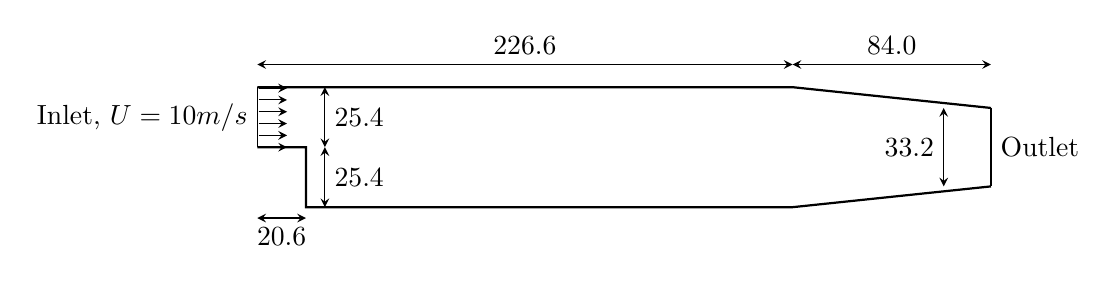
\begin{tikzpicture}[scale=0.03]
	% Draw the backward-facing step geometry
	\draw[thick] (-20.6,0) -- (0,0) -- (0,-25.4) -- (206,-25.4) -- (290,-16.6); % Lower
	\draw[thick] (-20.6,25.4) -- (0,25.4) -- (206,25.4) -- (290,16.6); % Upper
	\draw[thin] (-20.6,0) -- (-20.6,25.4) node[midway, left]{Inlet, $U = \qty{10}{m/s}$}; % Inlet
	\draw[thin] (290,-16.6) -- (290,16.6) node[midway, right]{Outlet}; % Outlet
	
	% Flow direction
	\foreach \y in {-0, 5, 10, 15, 20, 25} 
	\draw[-stealth] (-20,\y) -- ++(12,0);
	
	% Dimensions
	\draw[thin,stealth-stealth] (-20.6,35) -- (206,35) node[midway, above]{226.6}; 
	\draw[thin,stealth-stealth] (206,35) -- (290,35) node[midway, above]{84.0};
	\draw[thin,stealth-stealth] (270,-16.6) -- (270,16.6) node[midway, left]{33.2};
	\draw[thin,stealth-stealth] (8,0) -- (8,25.4) node[midway, right]{25.4};
	\draw[thin,stealth-stealth] (8,0) -- (8,-25.4) node[midway, right]{25.4};
	\draw[thin,stealth-stealth] (-20.6,-30) -- (0,-30) node[midway, below]{20.6};
\end{tikzpicture}
	\end{center}
	\caption{pitzDaily geometry. Lengths are in millimeter.}
\end{figure}

More information can be found on the \hyperlink{https://www.openfoam.com/documentation/tutorial-guide/3-compressible-flow/3.1-steady-turbulent-flow-over-a-backward-facing-step}{OpenFOAM website}.
\subsection{Governing Equations}
The \terminalcmd{pimpleFoam} solver implements the incompressible Reynolds-Averaged Navier-Stokes (RANS) equations:

\begin{equation}
\nabla \cdot \mathbf{U} = 0
\end{equation}

\begin{equation}
\frac{\partial \mathbf{U}}{\partial t} + \nabla \cdot (\mathbf{U} \mathbf{U})  = -\nabla \left(\frac{p}{\rho}\right) + \nabla \cdot (\nu_{\text{eff}} \nabla \mathbf{U})
\end{equation}

where $\nu_{\text{eff}} = \nu + \nu_t$ is the effective viscosity (molecular + turbulence viscosity).

Note that, since the fluid is incompressible,  instead of pressure $p$, this equation
deals with kinematic pressure , $\frac{p}{\rho}$, that has units of \unit{m^2/s^2}. 

\important{The solver \terminalcmd{pimpleFoam} keeps the name $p$ for the kinematic pressure.}

\subsection{Case Overview}
\begin{table}[h]
\centering
\begin{tabular}{@{}ll@{}}
\toprule
\textbf{Parameter} & \textbf{Value} \\
\midrule
Solver & \terminalcmd{pimpleFoam} (transient, incompressible) \\
Turbulence model & $k$-$\epsilon$ (standard) \\
Flow regime & Turbulent \\
Geometry & 2D backward-facing step \\
Reynolds number & $\sim 2 \times 10^4$ (based on step height) \\
Expected runtime & 20-40 seconds \\
\bottomrule
\end{tabular}
\caption{pitzDaily case specifications}
\label{tab:case_specs}
\end{table}

% ========== SECTION 2: TERMINAL SETUP ==========
\section{Terminal Environment Setup}

\subsection{Accessing OpenFOAM}
Open your terminal and verify OpenFOAM is available:

\begin{lstlisting}[style=terminal]
foamVersion
\end{lstlisting}

\important{If you see "command not found". you may need to source the OpenFOAM environment first:}
\begin{lstlisting}[style=terminal]
# For system-wide installation
source /usr/lib/openfoam/openfoam-2312/etc/bashrc
# For a local bash session with OpenFOAM
openfoam2512
\end{lstlisting}

\subsection{Navigating to Tutorials}
OpenFOAM includes a comprehensive set of tutorials. Navigate to the incompressible tutorials:

\begin{lstlisting}[style=terminal]
# Go to OpenFOAM tutorials directory
cd $FOAM_TUTORIALS

# List available tutorials
ls

# Navigate to incompressible pimpleFoam tutorials
cd incompressible/pimpleFoam
\end{lstlisting}

% ========== SECTION 3: CASE EXPLORATION ==========
\section{Case Structure Exploration}

\subsection{Understanding OpenFOAM Directory Structure}

Copy the pitzDaily case in a local folder

\begin{lstlisting}[style=terminal]
# Make a local folder
mkdir -p $HOME/Tutorials/Tutorial_1

# Copy the pitzDaily tutorial in this folder
cp -r ./pitzDaily $HOME/Tutorials/Tutorial_1

# Go to the tutorial place
cd $HOME/Tutorials/Tutorial_1
\end{lstlisting}

\important{Never play with a tutorial in the OpenFOAM distribution home folder. Always make a copy. In this way you will have always a "clean" copy.}

Examine the pitzDaily case structure:

\begin{lstlisting}[style=terminal]
# Go to the pitzDaily case
cd pitzDaily

# List all contents with details
ls -la

# See the directory structure
tree -L 2
\end{lstlisting}

\important{Every OpenFOAM case has this standard structure:}
\begin{lstlisting}[style=openfoam]
pitzDaily/
|-- 0/           # Initial and boundary conditions
|-- constant/    # Physical properties and mesh
|   |-- polyMesh/   # Mesh files
|   \-- transportProperties
\-- system/      # Solution control
    |-- controlDict
    |-- fvSchemes
    \-- fvSolution
\end{lstlisting}

\subsection{Examining Key Files}
Let's look at the most important configuration files:

\begin{enumerate}
	\renewcommand{\labelenumi}{\textbf{Step \arabic{enumi}:}}
\item \textbf{Initial Conditions (0/ directory)}:
\begin{lstlisting}[style=terminal]
# View velocity boundary conditions
cat 0/U

# View pressure boundary conditions  
cat 0/p

# View turbulence variables
cat 0/k
cat 0/epsilon
\end{lstlisting}

\item \textbf{Physical Properties}:
\begin{lstlisting}[style=terminal]
# Check fluid properties
cat constant/transportProperties
\end{lstlisting}

This shows:
\begin{lstlisting}[style=openfoam]
transportModel  Newtonian;

nu              1e-05;
\end{lstlisting}

\item \textbf{Solution Control}:
\begin{lstlisting}[style=terminal]
# Check solver settings
cat system/fvSolution

# Check discretization schemes
cat system/fvSchemes

# Check runtime control
cat system/controlDict
\end{lstlisting}
\end{enumerate}

\tip{Use \terminalcmd{less} or \terminalcmd{more} for longer files: \terminalcmd{less system/controlDict}}

% ========== SECTION 4: RUNNING THE SIMULATION ==========
\section{Running the Simulation}

\subsection{Pre-processing}
Before running, we need to generate the mesh:

\begin{lstlisting}[style=terminal]
# Generate the mesh using blockMesh, with the foamJob utility
foamJob -screen -log-app blockMesh

# Check mesh quality
foamJob -screen -log-app checkMesh
\end{lstlisting}

\warning{If \terminalcmd{blockMesh} fails, check for error messages. Common issues include missing dictionaries or syntax errors in \filename{system/blockMeshDict}.}

The utility \terminalcmd{foamJob} creates a log file.
 
\begin{lstlisting}[style=terminal]
# Check the content of the log files
less log.blockMesh
less log.checkMesh
\end{lstlisting}

\subsection{Running pimpleFoam}
Now run the simulation:

\begin{lstlisting}[style=terminal]
# Run the solver
foamJob -s -log-app pimpleFoam

\end{lstlisting}

\subsection{Monitoring Convergence}
Monitor convergence:

\begin{lstlisting}[style=terminal]
# Watch residuals in real-time (if running in foreground)
# OR check the log file periodically:

# Show last 20 lines of residuals
tail -20 log.pimpleFoam | grep "Solving for"

# Check final residuals
tail -50 log.pimpleFoam | grep "Final residual"
\end{lstlisting}

Plot it using \terminalcmd{gnuplot}

\begin{lstlisting}[style=terminal]
# Generate residual files from the log file
foamLog log.pimpleFoam

# Visualize the residuals of the main variables with gnuplot
gnuplot
gnuplot> set logscale y
gnuplot> plot  'logs/p_0'with lines ,'logs/Ux_0' with lines, 'logs/Uy_0' with lines, 'logs/epsilon_0' with lines, 'logs/k_0' with lines
\end{lstlisting}

You will get a picture similar to that in Figure \ref{fig:gnuplot}.

\begin{figure}[h]
	\centering
	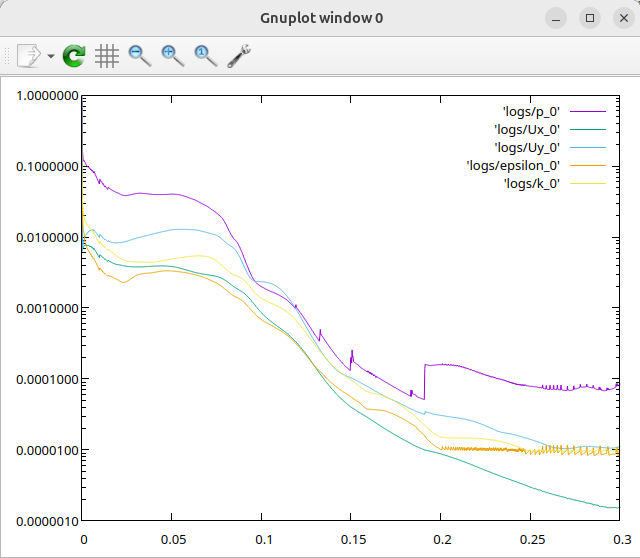
\includegraphics[width=0.7\linewidth]{gnuplot}
	\caption{Plot of residuals}
	\label{fig:gnuplot}
\end{figure}

% ========== SECTION 5: POST-PROCESSING ==========
\section{Post-Processing in Terminal}

\subsection{Basic Results Examination}
OpenFOAM stores results in time directories. Examine the final results:

\begin{lstlisting}[style=terminal]
# List time directories
foamListTimes

# Go to final time directory (0.3 for this simulation)
cd 0.3

# List available fields
ls

\end{lstlisting}

\subsection{Using OpenFOAM Command Line Tools}


\begin{itemize}
	\item Check field statistics



\begin{lstlisting}[style=terminal]
# Go back to case root if you are still in the time folder
cd ..

# Get some statistics
postProcess -func writeCellCentres
postProcess -func minMaxMagnitude
\end{lstlisting}

\item Check average pressure in inlet:

\begin{lstlisting}[style=terminal]
# Get the dictionary 
foamGetDict patchAverage
\end{lstlisting}

This will add the file \filename{system/patchAverage} to the case. The name of this function can be changed, and it can be edited to define the patch and the variable to be averaged

\begin{lstlisting}[style=terminal]
# Rename the function 
mv system/patchAverage system/inletAveragePressure
# Edit the function (you can use vim, nano, emacs, ...)
vim system/inletAveragePressure
\end{lstlisting}

\begin{lstlisting}[style=output]
...
name    inlet;
fields  (p);

operation areaAverage;
#includeEtc "caseDicts/postProcessing/surfaceFieldValue/patch.cfg"
...
\end{lstlisting}

\begin{lstlisting}[style=terminal]
# compute average pressure in inlet 
postProcess -func inletAveragePressure
\end{lstlisting}

\end{itemize}

\tip{The command \terminalcmd{postProcess -list} will list all the functions available.}

Besides the screen, the information from \terminalcmd{postProcess} is also saved in the 
\filename{postProcessing} folder. In order to plot the results of a post-processing 
function (pressure average in inlet patch, for instance), the utility 
\terminalcmd{foamMonitor} is used

\begin{lstlisting}[style=terminal] 
foamMonitor postProcessing/inletAveragePressure/0.3/surfaceFieldValue.dat
\end{lstlisting}

\begin{figure}[H]
	\centering
	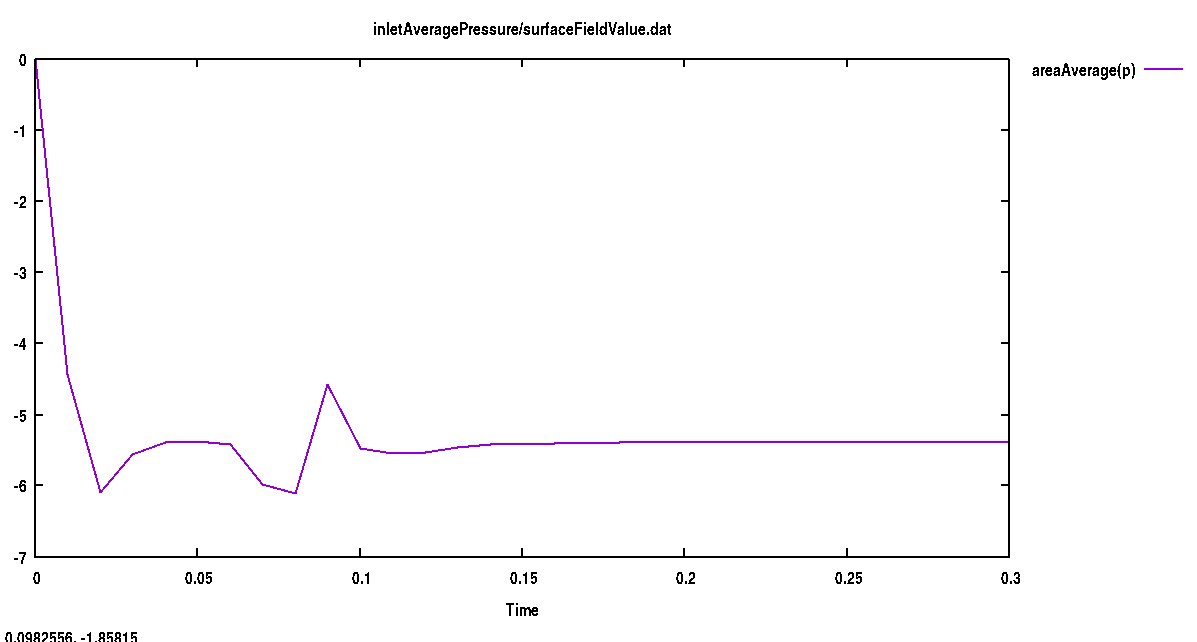
\includegraphics[width=\linewidth]{foamMonitorPressure}
	\caption[Monitoring average pressure in inlet]{}
	\label{fig:foammonitorpressure}
\end{figure}

\subsection{Plotting residuals}

In the last section we have seen how to monitor residuals from the log file. But it is also possible to save the residuals in a data-file in order to post-process them with \terminalcmd{foamMonitor} or any other application (a Python script, for instance)

In order to log the residuals in run time, the function has to be added in the \filename{system} folder with

\begin{lstlisting}[style=terminal]
foamGetDict solverInfo
\end{lstlisting} 

It will give two options. Usually it is better the first one.

\subsubsection{Runtime post-processing and monitoring}

Let's run again the previous simulation, but this time with computation, in run-time, of
\begin{enumerate}
	\item Residuals
	\item Total pressure
	\item Average of total pressure in inlet and outlet
	\item Vorticity and second invariant of velocity gradient tensor, $Q$
	\item Wall shear stress and $y^+$
\end{enumerate} 

Go back to the case root and clean it

\begin{lstlisting}[style=terminal]
foamListTimes -rm
\end{lstlisting} 

Get the required dictionaries

\begin{lstlisting}[style=terminal]
# Get the function to record residuals
foamGetDict solverInfo
# Get the function to compute toal pressure
foamGetDict totalPressureIncompressible
# Get the functions to compute total pressure in inlet and outlet
foamGetDict patchAverage
# move this file to a personalized function for inlet patch
mv system/patchAverage system/inletTotalPressureAverage
# copy this file for the oulet patch
cp system/inletTotalPressureAverage system/outletTotalPressureAverage
# Get the functions to compute vorticity, Q, wall shear stress and yPlus
foamGetDict vorticity
foamGetDict Q
foamGetDict wallShearStress
foamGetDict yPlus
\end{lstlisting} 

Edit the function files to fit the simulation requirements. 

The \filename{system/solverInfo} should look like that:

\begin{lstlisting}
#includeEtc "caseDicts/postProcessing/numerical/solverInfo.cfg"

fields (p U k omega);
\end{lstlisting} 

The \filename{system/totalPressureIncompressible} is like that:
\begin{lstlisting}
#includeEtc "caseDicts/postProcessing/pressure/totalPressureIncompressible.cfg"

pRef    0.0;
rhoInf  1.2;

executeControl timeStep;
\end{lstlisting}

Change the density in function of the fluid. The keyword for \ofkeyword{executeControl} is included in order the compute total pressure in every time step, to compute average values in the next
functions. If this statement is not included, by default it is executed and written just in the \ofkeyword{writeTime}, i.e. in the times when fields are written fo disc.
The \\
\filename{system/inletTotalPressureAverage} file
is like that:

\begin{lstlisting}
name    inlet;
fields  (total(p));

operation areaAverage;
#includeEtc "caseDicts/postProcessing/surfaceFieldValue/patch.cfg"
\end{lstlisting} 

and the file \filename{system/inletTotalPressureAverage} is the same, but with the 
\texttt{name outlet;} statement. The functions \filename{system/vorticity}, 
\filename{system/Q}, \filename{system/wallShearStress} and 
\filename{system/yPlus} have to be
kept unmodified.

Finally, in order the solver to read all this functions, they have to be included in the \filename{system/controlDict} file. Include this at the end of the file:

\begin{lstlisting}
functions{
	#includeFunc solverInfo
	#includeFunc totalPressureIncompressible
	#includeFunc inletTotalPressureAverage
	#includeFunc outletTotalPressureAverage	
	#includeFunc vorticity
	#includeFunc Q
	#includeFunc wallShearStress
	#includeFunc yPlus
}

\end{lstlisting} 

Run the solver again with
\begin{lstlisting}[style=terminal]
foamJob -s -log-app pimpleFoam
\end{lstlisting}
and monitor the residuals with
\begin{lstlisting}[style=terminal]
foamMonitor -l postProcessing/solverInfo/0/solverInfo.dat
\end{lstlisting}

\warning{The option \terminalcmd{-l} is to plot $y$-axes with logarithm scale.}

The output should be similar to Figure \ref{fig:residuals}


\begin{figure}[H]
	\centering
	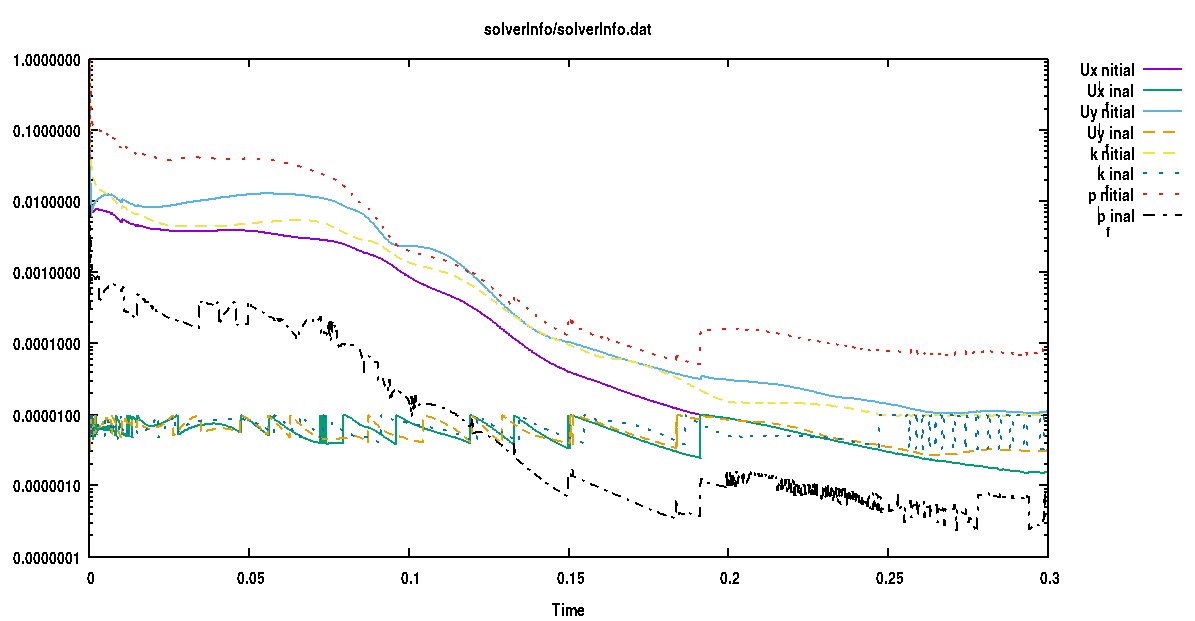
\includegraphics[width=1\linewidth]{residuals}
	\caption{Plot of residuals with \terminalcmd{foamMonitor}.}
	\label{fig:residuals}
\end{figure}

Plot time evolution of total pressure in inlet
\begin{lstlisting}[style=terminal]
foamMonitor postProcessing/inletTotalPressureAverage/0/surfaceFieldValue.dat
\end{lstlisting}
and outlet
\begin{lstlisting}[style=terminal]
foamMonitor postProcessing/outletTotalPressureAverage/0/surfaceFieldValue.dat
\end{lstlisting}

\begin{figure}[H]
	\centering
	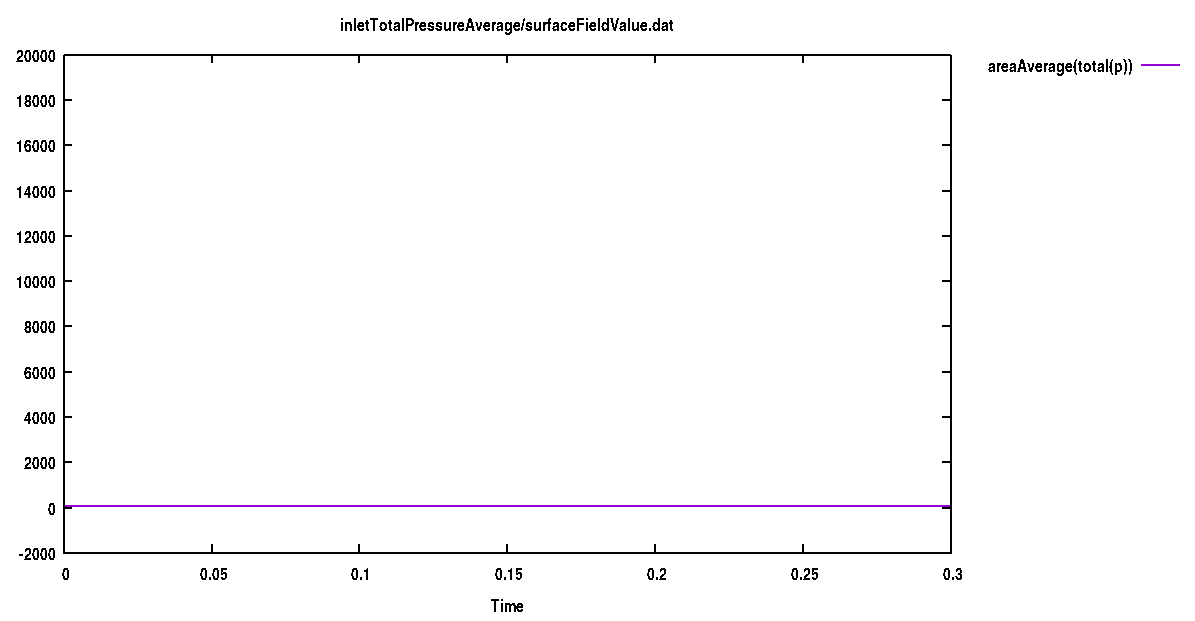
\includegraphics[width=1\linewidth]{inletTotalPressure}
	\caption{Inlet total pressure}
	\label{fig:inlettotalpressure}
\end{figure}
\begin{figure}
	\centering
	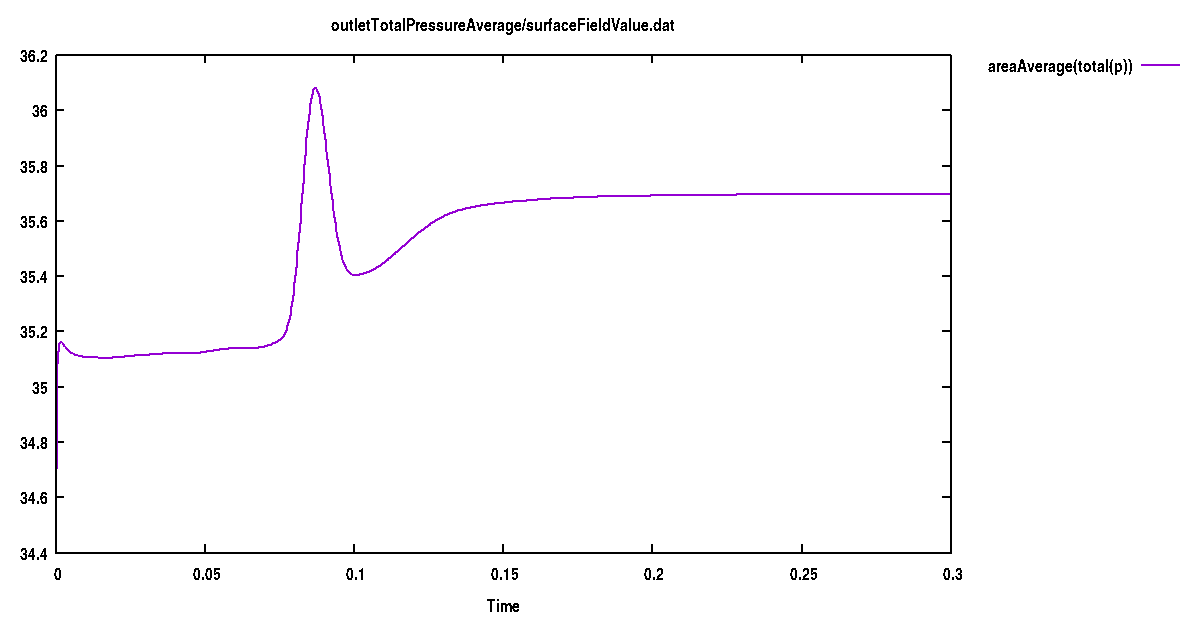
\includegraphics[width=1\linewidth]{outletTotalPressure1}
	\caption{Outlet total pressure}
	\label{fig:outlettotalpressure1}
\end{figure}

The specific values for the total pressures in outlet and inlet can be obtained for the
text files

\begin{lstlisting}[style=terminal]
tail -200 postProcessing/inletTotalPressureAverage/0/surfaceFieldValue.dat
\end{lstlisting}

\begin{lstlisting}[style=output]
...
0.29          	5.354488e+01
0.290256      	5.354490e+01
0.290513      	5.354492e+01
0.290769      	5.354493e+01
0.291026      	5.354494e+01
0.291282      	5.354496e+01
0.291538      	5.354497e+01
0.291795      	5.354498e+01
0.292051      	5.354499e+01
0.292308      	5.354500e+01
0.292564      	5.354501e+01
0.292821      	5.354508e+01
0.293077      	5.354507e+01
0.293333      	5.354509e+01
0.29359       	5.354508e+01
0.293846      	5.354500e+01
0.294103      	5.354520e+01
0.294359      	5.354525e+01
0.294615      	5.354525e+01
0.294872      	5.354526e+01
0.295128      	5.354527e+01
0.295385      	5.354528e+01
0.295641      	5.354529e+01
0.295897      	5.354530e+01
0.296154      	5.354530e+01
0.29641       	5.354531e+01
0.296667      	5.354531e+01
0.296923      	5.354532e+01
0.297179      	5.354532e+01
0.297436      	5.354532e+01
0.297692      	5.354533e+01
0.297949      	5.354534e+01
0.298205      	5.354534e+01
0.298462      	5.354535e+01
0.298718      	5.354535e+01
0.298974      	5.354511e+01
0.299231      	5.354531e+01
0.299487      	5.354532e+01
0.299744      	5.354533e+01
0.3           	5.354533e+01
\end{lstlisting}

\begin{lstlisting}[style=terminal]
	tail -200 postProcessing/outletTotalPressureAverage/0/surfaceFieldValue.dat
\end{lstlisting}

\begin{lstlisting}[style=output]
...
0.29          	3.569808e+01
0.290256      	3.569808e+01
0.290513      	3.569808e+01
0.290769      	3.569809e+01
0.291026      	3.569809e+01
0.291282      	3.569809e+01
0.291538      	3.569809e+01
0.291795      	3.569809e+01
0.292051      	3.569810e+01
0.292308      	3.569810e+01
0.292564      	3.569810e+01
0.292821      	3.569810e+01
0.293077      	3.569810e+01
0.293333      	3.569811e+01
0.29359       	3.569811e+01
0.293846      	3.569811e+01
0.294103      	3.569811e+01
0.294359      	3.569811e+01
0.294615      	3.569811e+01
0.294872      	3.569812e+01
0.295128      	3.569812e+01
0.295385      	3.569812e+01
0.295641      	3.569812e+01
0.295897      	3.569812e+01
0.296154      	3.569812e+01
0.29641       	3.569812e+01
0.296667      	3.569813e+01
0.296923      	3.569813e+01
0.297179      	3.569813e+01
0.297436      	3.569813e+01
0.297692      	3.569813e+01
0.297949      	3.569813e+01
0.298205      	3.569814e+01
0.298462      	3.569814e+01
0.298718      	3.569814e+01
0.298974      	3.569814e+01
0.299231      	3.569814e+01
0.299487      	3.569814e+01
0.299744      	3.569814e+01
0.3           	3.569815e+01
\end{lstlisting}

Així doncs, $p_{0,i} = \qty{53.5}{Pa}$, and $p_{0,o} = \qty{35.7}{Pa}$ and
\begin{equation}
	\Delta p_0 = \qty{17.8}{Pa}
\end{equation}
and the dimensionless pressure loss coefficient is
\begin{equation}
	k = \frac{\Delta p_0}{\frac{1}{2} \rho U^2} = 0.3
\end{equation}

\section{Basic Visualization in paraview}
Usually the program \terminalcmd{paraview} is used to visualize the results from OpenFOAM simulations. A wrapper \terminalcmd{paraFoam} is available to call the 
program after performing some internal operations


\begin{lstlisting}[style=terminal]
# Run the paraFoam script
paraFoam
\end{lstlisting}

\begin{figure}[H]
	\centering
	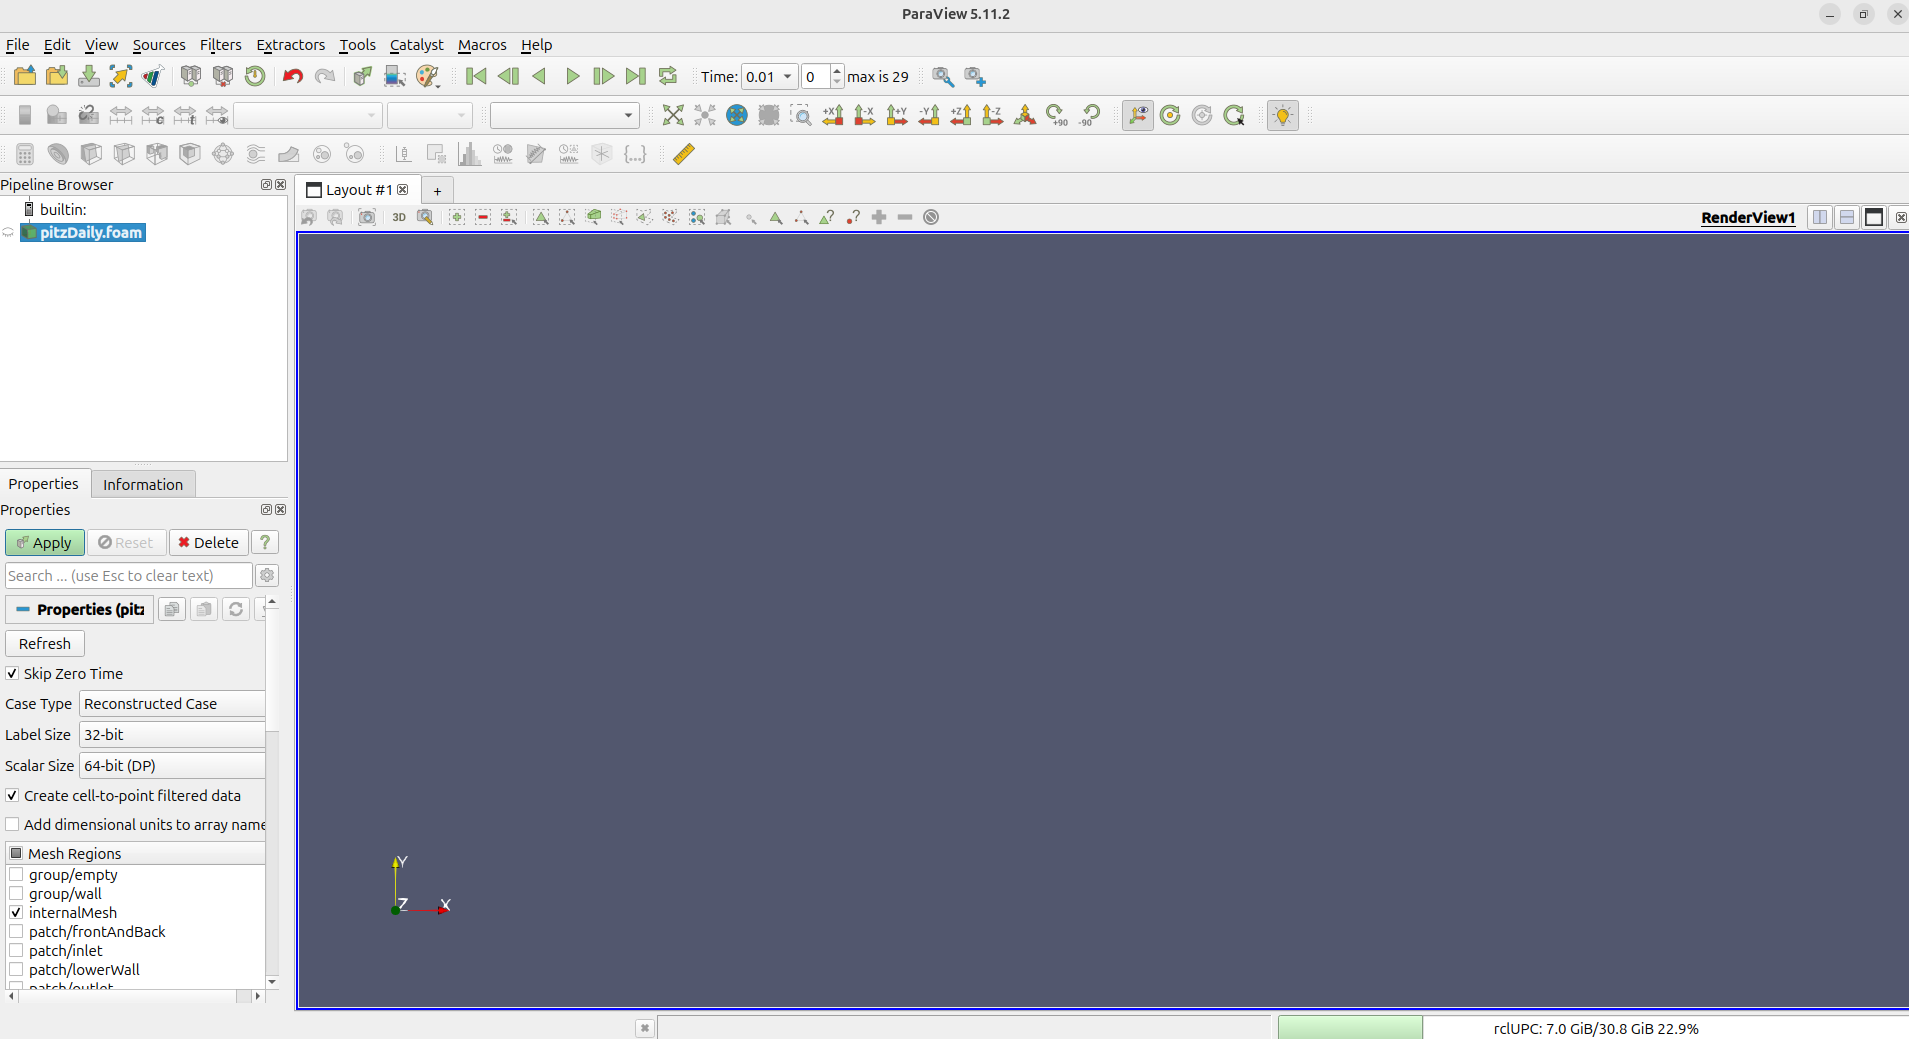
\includegraphics[width=\linewidth]{paraFoam001}
	\caption{Start screen for paraview, called with \terminalcmd{paraFoam}.}
	\label{fig:parafoam001}
\end{figure}

Click on the \ofkeyword{Apply}  button. By default, you will the pressure distribution (Figure \ref{fig:parafoam002}).

\begin{figure}[H]
	\centering
	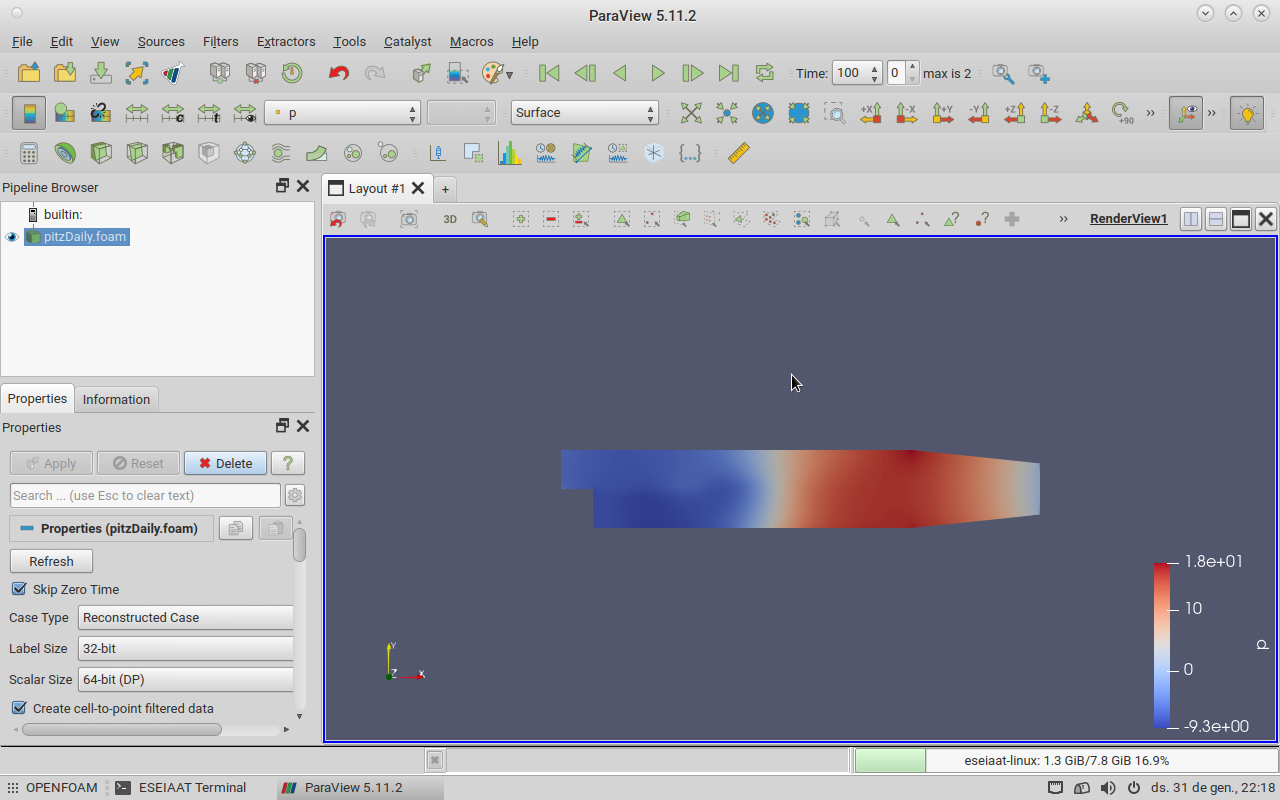
\includegraphics[width=\linewidth]{paraFoam002}
	\caption{Pressure distribution of the flow.}
	\label{fig:parafoam002}
\end{figure}

Click on the \ofkeyword{Play} button to see the time evolution of pressure distribution.

Switch the displayed variable to $Q$ 
\includegraphics{Q_icon}. Note that the range is
huge both for the positive and negatives values. This  is due to the high gradients
of velocity in the inlet zone close to the walls. The uniform value of the inlet 
velocity generates the strong derivatives in the regions close to the solid walls. 
The actual value of $Q$ in the fluid domain ranges approximately from -10000 to 10000.
The displayed range can be modified in the \terminalcmd{Rescale to Custom Data Range}
tool.  Result is shown in figure \ref{fig:parafoamq}, where to strong vortex, 
identified by positive values of $Q$, is placed 
just after the back-step.

\begin{figure}[H] 			
	\centering
	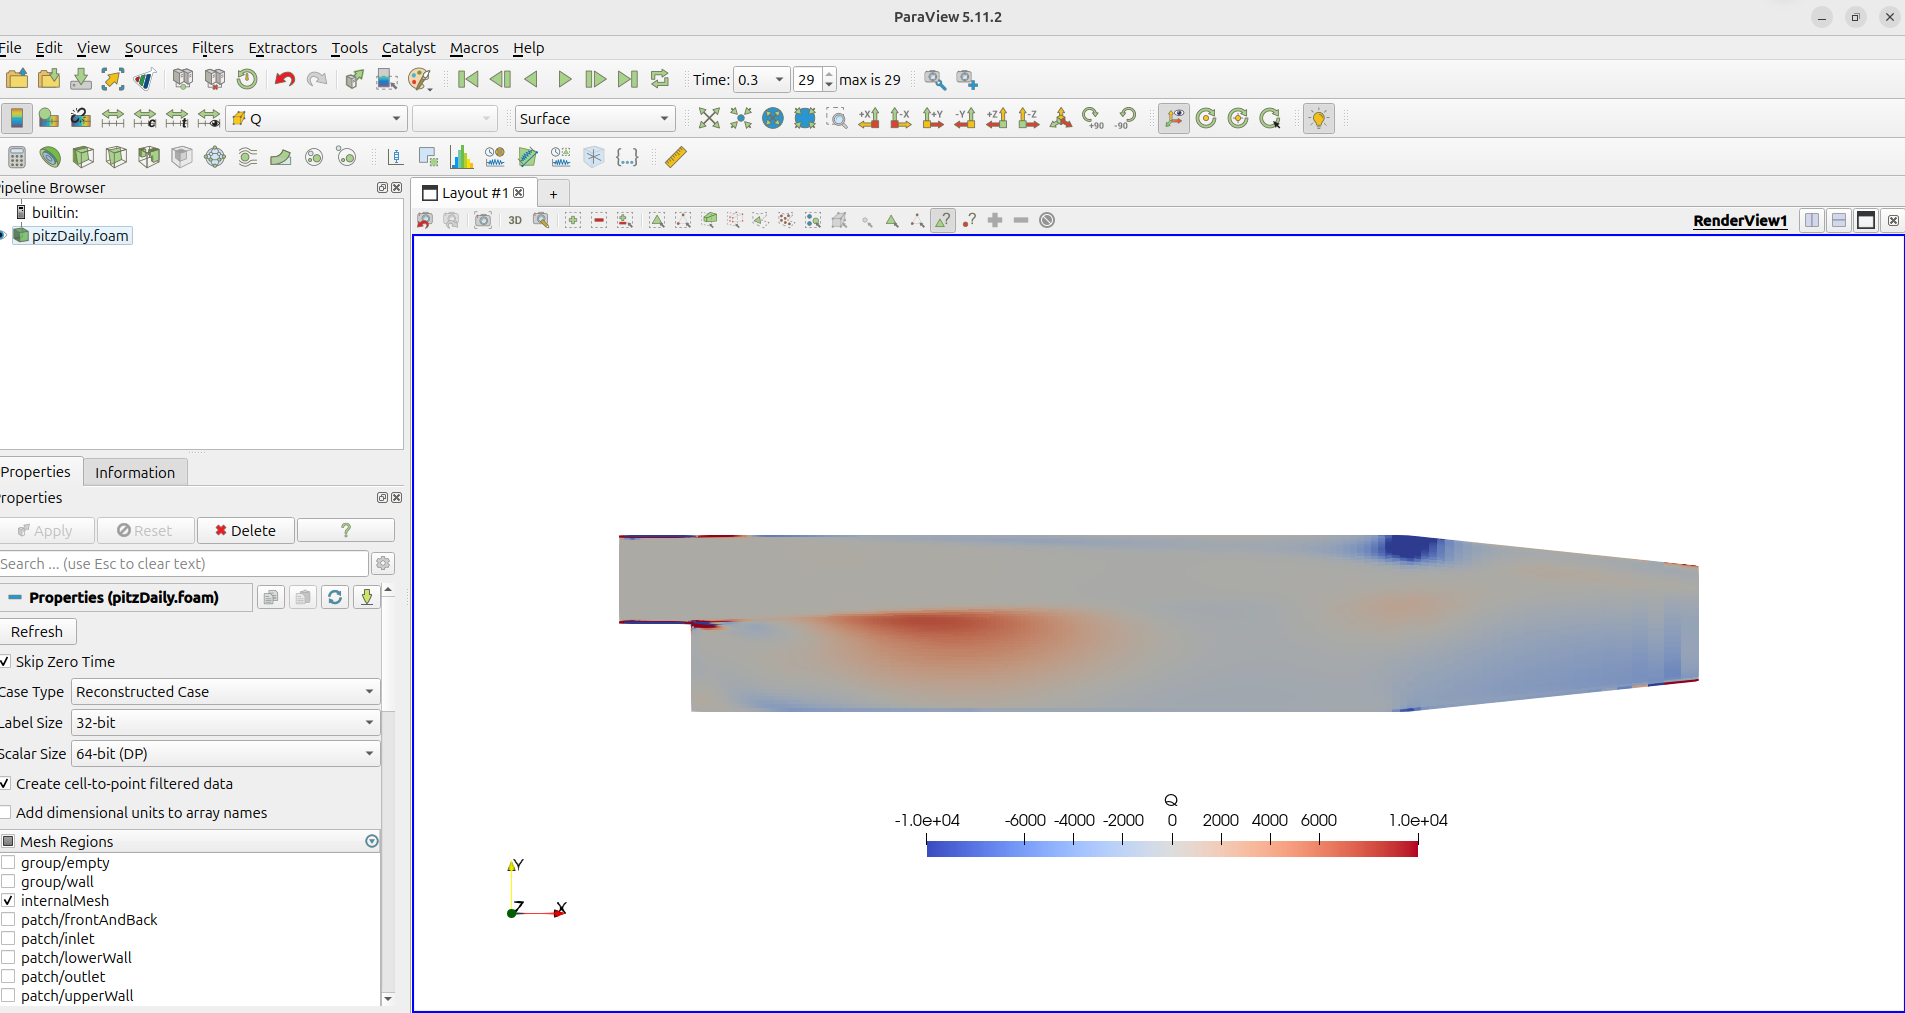
\includegraphics[width=1\linewidth]{paraFoam_Q}
	\caption{Distribution of $Q$}
	\label{fig:parafoamq}
\end{figure}

Figure \ref{fig:streamlines} shows the flow streamlines. This is obtained with the 
\terminalcmd{Stream Tracer} filter, placing the line, parallel to the $y$-axis, in 
$x = \qty{0.07}{m}$ and with a resolution of 100 lines.

\begin{figure}[H]
	\centering
	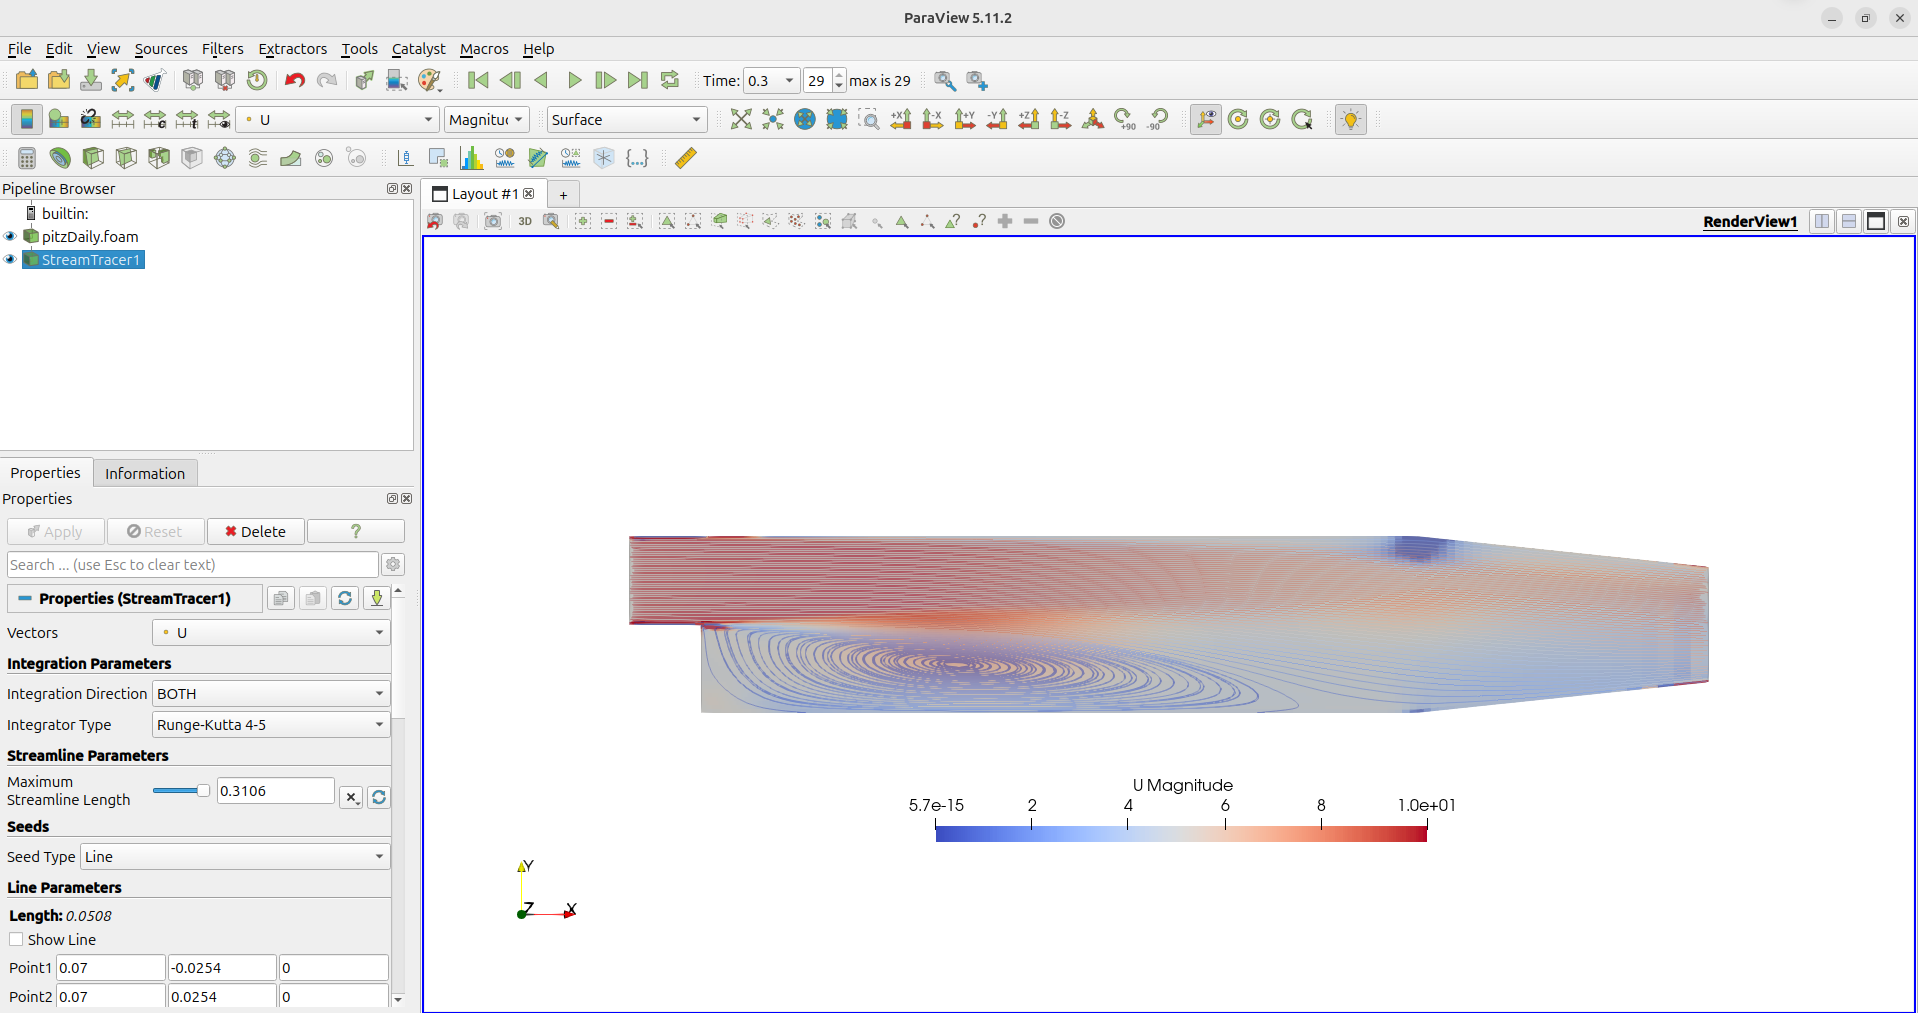
\includegraphics[width=\linewidth]{streamLines}
	\caption{Flow streamlines. The background is the $Q$ distribution.}
	\label{fig:streamlines}
\end{figure}
´
Let's we now identify the exact point of reattachment of the flow after the step. 

In the main item in the \terminalcmd{Pipeline browser} select only 
the \texttt{patch/lowerWall} in \terminalcmd{Mesh Regions}. In the screen only 
this patch will be visible. In the \terminalcmd{Filter - Data Analysis} menu, select
\terminalcmd{Plot Data}. A new window will be created in the canvas, with plots of
the main variables in this patch.

Unable the \terminalcmd{Use Index as XAxis} tick and select \terminalcmd{Points\_X} as 
\terminalcmd{X Array Name}. Result is shown in Figure \ref{fig:wallshearstressplot}.
Note that flow is reattached when the sign of the shear stress changes from positive 
to negative, in $x=\qty{180}{mm}$.


\begin{figure}[H]
	\centering
	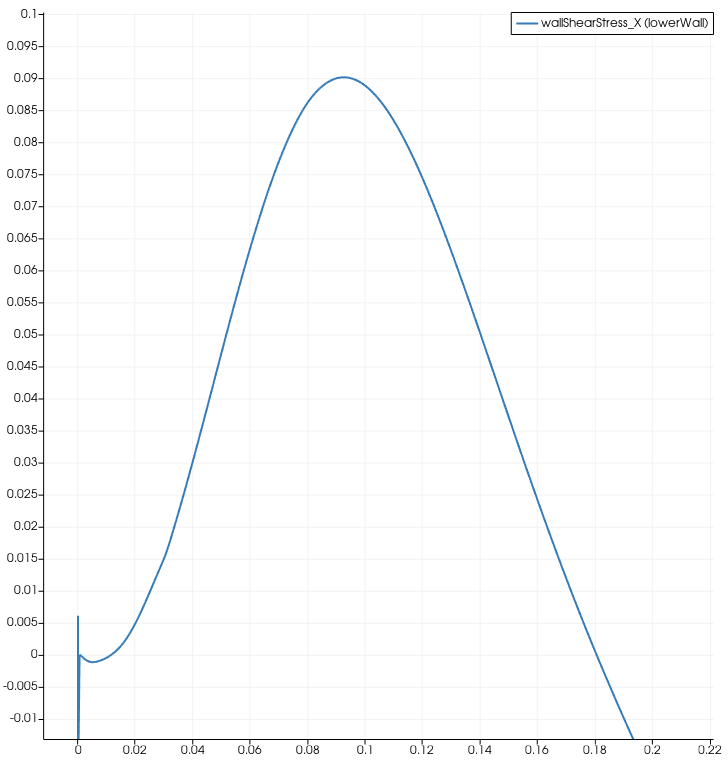
\includegraphics[width=\linewidth]{wallShearStress_Plot}
	\caption{Plot of wall shear stress in the lower wall patch.}
	\label{fig:wallshearstressplot}
\end{figure}

Finally, we plot the value of $y^+$ for both lower and upper walls 
(Figure \ref{fig:yplus}). Note that, specially for upper wall, the value of $y^+$ falls
inside the laminar sub-layer ( $y^+ \lessapprox 11$ ). This is handled by the wall
function defined in \filename{0/nut} by imposing $\nu_t = 0$ in order to avoid
overestimation of the wall shear stress. 

\begin{figure}[H]
	\centering
	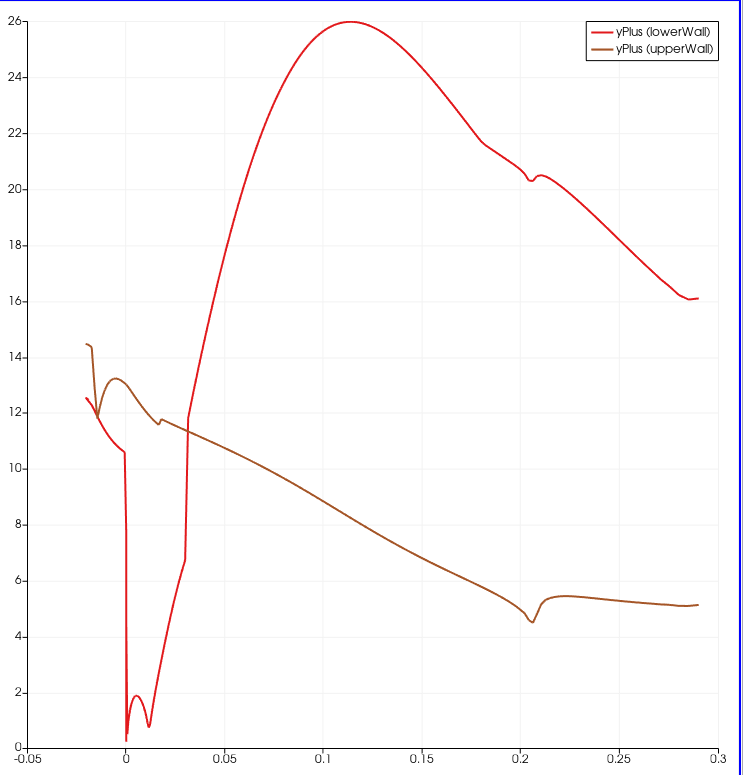
\includegraphics[width=\linewidth]{yPlus}
	\caption{Plor y $y^+$ distribution in upper and lower walls.}
	\label{fig:yplus}
\end{figure}


% ========== SECTION 6: TROUBLESHOOTING ==========
\section{Common Issues and Troubleshooting}

\subsection{Error: "command not found"}
\begin{itemize}
\item \textbf{Cause}: OpenFOAM environment not sourced
\item \textbf{Solution}: 
\begin{lstlisting}[style=terminal]
source /usr/lib/openfoam/openfoam2512/etc/bashrc
# or just 
openfoam2512
\end{lstlisting}
\end{itemize}

\subsection{Error: "cannot find blockMeshDict" (or any other dictionary)}
\begin{itemize}
\item \textbf{Cause}: Not in correct directory or file missing
\item \textbf{Solution}:
\begin{lstlisting}[style=terminal]
# Check current directory
pwd

# List contents of system
ls system
\end{lstlisting}
\end{itemize}

\subsection{Simulation Diverges (Residuals Grow)}
\begin{itemize}
\item \textbf{Cause}: Poor initial conditions or solver settings
\item \textbf{Solution}:
\begin{enumerate}
\item Reduce under-relaxation factors in \filename{system/fvSolution}
\item Check boundary conditions are physically realistic
\item Try running \terminalcmd{potentialFoam} first to get better initial fields
\end{enumerate}
\end{itemize}


% ========== SECTION 7: EXERCISES ==========
\section{Student Exercises and Extensions}

\subsection{Basic Exercises}
\begin{enumerate}

\item \textbf{Boundary Condition Modification}:
\begin{itemize}
\item Change inlet velocity from \SI{10}{\meter\per\second} to \SI{20}{\meter\per\second}
\item Update both \filename{0/U} and \filename{0/k}/\filename{0/epsilon} appropriately
\item \textbf{Question}: How does Reynolds number affect recirculation zone size?
\end{itemize}

\item \textbf{Turbulence Model Comparison}:
\begin{itemize}
\item Change from $k$-$\epsilon$ to $k$-$\omega$ SST in \filename{constant/turbulenceProperties}

Use the command \terminalcmd{foamCloneCase} to copy a "naked" case. 

\tip{You will have to change several files. Check some tutorial with this turbulence
model for information. }

\tip{For computation of turbulence variables, you can see this 
	\hyperlink{https://www.cfd-online.com/Wiki/Turbulence_free-stream_boundary_conditions}{web page in CFD online}. Get a relationship between $\varepsilon$ and $\omega$
	from the expression in this web page. The computation of the new field can be done with the proper dictionary. See examples in \\
	 \filename{\$FOAM\_TUTORIALS/incompressible/pisoFoam/RAS/cavity/system/FOs}}
\item \textbf{Question}: Which model converges faster? Which gives higher $k$ values? Is the dimensionless pressure loss coefficient changing?
\end{itemize}
\end{enumerate}

\subsection{Advanced Exercises (Optional)}
\begin{enumerate}
\item \textbf{Mesh Refinement Study}:
\begin{itemize}
\item Modify \filename{system/blockMeshDict} to double cells in x-direction
\item Compare velocity profiles at outlet
\end{itemize}
\end{enumerate}

% ========== APPENDIX ==========
\appendix
\section{Appendix: Useful Terminal Commands Reference}

\subsection{OpenFOAM-Specific}
\begin{tabular}{@{}ll@{}}
\toprule
\textbf{Command} & \textbf{Purpose} \\
\midrule
\terminalcmd{foamJob} & Run an openfoam command saving the log file \\
\terminalcmd{blockMesh} & Generate block-structured mesh \\
\terminalcmd{checkMesh} & Check mesh quality \\
\terminalcmd{simpleFoam} & Run steady incompressible solver \\
\terminalcmd{foamLog} & Parse log file for residuals \\
\terminalcmd{postProcess} & Execute function objects \\
\terminalcmd{paraFoam} & Launch visualization (if GUI available) \\
\terminalcmd{reconstructPar} & Reconstruct parallel case \\
\bottomrule
\end{tabular}

\subsection{General Linux Commands}
\begin{tabular}{@{}ll@{}}
\toprule
\textbf{Command} & \textbf{Purpose} \\
\midrule
\terminalcmd{grep "keyword" file} & Search for text in file \\
\terminalcmd{tail -f log} & Follow log file in real-time \\
\terminalcmd{head -n 20 file} & Show first 20 lines \\
\terminalcmd{cd \textasciitilde/} & Go to home directory \\
\terminalcmd{pwd} & Print working directory \\
\terminalcmd{ls -la} & List all files with details \\
\terminalcmd{tree -L 2} & Show directory tree (2 levels) \\
\bottomrule
\end{tabular}

\section{Quick Reference: File Locations in pitzDaily}
\begin{itemize}
\item \textbf{Mesh definition}: \filename{constant/polyMesh/blockMeshDict}
\item \textbf{Boundary conditions}: \filename{0/U}, \filename{0/p}, \filename{0/k}, \filename{0/epsilon}
\item \textbf{Solver settings}: \filename{system/fvSolution}
\item \textbf{Discretization schemes}: \filename{system/fvSchemes}
\item \textbf{Runtime control}: \filename{system/controlDict}
\item \textbf{Material properties}: \filename{constant/transportProperties} 
\item \textbf{Turbulence model}: \filename{constant/turbulenceProperties}
\end{itemize}

% ========== DISCLAIMER ============

\section*{Disclaimer}

This tutorial has been developed by \textbf{Robert Castilla}, 
of the Departament of Fluid
Mechanics in the Universitat Politècnica de Catalunya, for the doctoral 
workshop at \textbf{IMP⁻PAN Gda\'{n}sk} (July 2026). The author utilized \textbf{DeepSeek} for the initial
definition of the document format. Further technical refinement and the development
of advanced post-processing exercises were supported by \textbf{NotebookLM}. All the technical
information for the \textbf{OpenFOAM v2512} environmnet and all physical interpretations were
performed and approved by the author. 

% ========== END DOCUMENT ==========
\end{document}